\subsection{Mecanismos de Atención}

Una de las arquitecturas comunes vistas previamente es la \ref{fig:rnn_cfgc} cuya información
procesada es resumida en una sola salida. Este tipo de red es usada como parte de las soluciones a
tareas de como reconocimiento de voz (\textit{Speech Recognition}), traducción de lenguaje
(\textit{Machine Translation}) o asistencia en respuestas automáticas (\textit{Question Answering})
típicamente bajo modelos Secuencia a Secuencia (\textit{Sequence to Sequence, Seq2Seq}). Los modelos
\textit{Seq2Seq} están formados por dos redes neuronales como la mostrada en \ref{fig:seq2seq}. La
primera se comporta como \textit{codificador} al resumir la entrada para producir un vector de salida
de tamaño fijo llamado \textit{vector de contexto}. La segunda red se comporta como un
\textit{decodificador}, este es inicializado y condicionado con el
\textit{vector de contexto} para obtener una transformación de la entrada no necesariamente del
mismo tamaño de secuencia, ya sea por ejemplo, traducir una oración de español a inglés en donde la
traducción no siempre contiene las misma cantidad de palabras usadas en el idioma original.

\begin{figure}[ht!]
    \centering
    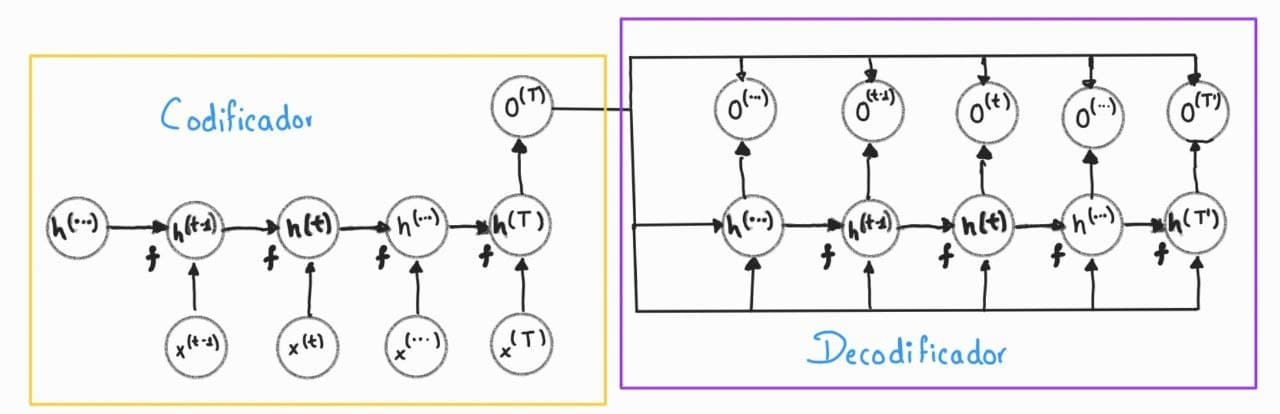
\includegraphics[width=1.0 \textwidth]{Chapters/1. Transformer/Figures/rnn/seq2seq.jpg}
    \caption{Descripción.}
    \label{fig:seq2seq}
\end{figure}

Por ejemplo, en tareas de \textit{Machine Translation} el \textit{encoder} esta formado por una
\textit{RNN} Bidireccional que lee y procesa un conjunto de
vectores $X = (x^{(1)}, x^{(2)}, \dots, x^{(T_x)})$ para obtener un vector de contexto $C$. La forma
más común es como en \ref{eq:s2s_simple}:

\begin{equation}
    \begin{split}
        h^{(t)} = f_{bi}(x^{(t)}, h^{(t-1)}; \theta_{f}, \theta_{b}) \\
        C = q({h^{(1)}, h^{(2)}, \dots, h^{(T)}})
    \end{split}
    \label{eq:s2s_simple}
\end{equation}

Recordemos que $h^{(t)}$ es el estado oculto generado por la concatenación de los dos estados ocultos
generados por la \textit{RNN Bidireccional}, $f_{bi}$ y $q$ son funciones no lineales, ya sea,
una \textit{LSTM} para $f_{bi}$ y $q({h^{(1)}, h^{(2)}, \dots, h^{(T)}}) = h^{(T)}$, equivalente a
tomar solo el ultimo estado oculto como vector de contexto $C$. El \textit{Decoder} es entrenado
para predecir la siguiente palabra $y^{(t')}$ dado el vector de contexto $C$ y todas las palabras
previas predichas. En otras palabras, el decoder define la probabilidad conjunta modelada por una
\textit{RNN}:

\begin{equation}
    p(Y) = \prod_{t=1}^{T_y} p(y^{(t)} | \{y^{(1)}, \dots , y^{(t-1)}\}, C)
\end{equation}
\begin{equation}
    p(y^{(t)} | \{y^{(1)}, \dots , y^{(t-1)}\}, C) = g(y^{(t-1)}, s^{(t)}, C; \theta_g)
\end{equation}

donde $g$ es una función no lineal que emite la probabilidad de $y^{(t)}$ y $s^{(t)}$ es el estado oculto
del \textit{decoder} \ref{eq:sqs_s}.

\begin{equation}
    s^{(t)} = f(s^{(t)}, y^{(t-1)}, C; \theta_s)
    \label{eq:sqs_s}
\end{equation}


Sin embargo, cuando las secuencias son bastante largas el \textit{vector de contexto} emitido por el
\textit{codificador} no es lo suficientemente grande como para resumir correctamente la secuencia y
por tanto, la información inicial de la entrada es olvidad, por lo que su presencia es escasa en estados
ocultos más lejanas. Así, en 2015 \cite[Bahdanau et. al]{bahdanau2016neural} observaron estos efectos y
propusieron una forma de minimizarlos, surgiendo los \textbf{Mecanismos de Atención}.

Ahora las palabras predichas no son calculadas por un único \textit{vector de contexto} generado por
el codificador, sino que para cada objetivo $y^{(t)}$ se calcula un \textit{vector de contexto} $c^{(t)}$:

\begin{equation}
    p(y^{(t)} | \{y^{(1)}, \dots , y^{(t-1)}\}, c^{(t)}) = g(y^{(t-1)}, s^{(t)}, c^{(t)}; \theta_g)
\end{equation}

\begin{equation}
    s^{(t)} = f(s^{(t)}, y^{(t-1)}, c^{(t)}; \theta_s)
\end{equation}

Dado que cada estado oculto $h^{(t)}$ contiene mucho mejor la información que se encuentran alrededor
del t-ésimo término, se puede generar cada vector de contexto como una suma pesada de sobre los
estados ocultos del codificador. Estos pesos nos ayudan a determinar que tan importante es la
información codificada por cada estado oculto y al momento de obtener la salida del t-ésimo valor
\quotes{prestar atención} a aquellos que son más relevantes para obtener la predicción:

\begin{equation}
    c^{(t)} = \sum_{i=1}^{T_x} \alpha_{t,i} h^{(i)}
\end{equation}

cada peso $\alpha_{t,i}$ indica que tan bien se \quotes{alinean} los términos $y^{(t)}$ y $x^{(i)}$

\begin{equation}
    \alpha_{t,i} = align(y^{(t)}, x^{(i)}) = \frac{\exp(score(s^{(t-1)}, h^{(i)}))}{\sum_{k=1}^{T_x} \exp(score(s^{(t-1)}, h^{(k)}))}
\end{equation}

\textit{Bahdanau} propone aprender esta alineación usando una \textit{Red feed-forward} con una sola
capa oculta y la función $\tanh$ como activación:

\begin{equation}
    score(s^{(t)}, h^{(i)}) = v^\top_a \tanh(W_a[s^{(t)};h^{(i)}])
\end{equation}

con $v_a$ y $W_a$ como matrices de pesos a aprender durante el entrenamiento. En la figura \ref{fig:att}
podemos ver gráficamente el modelo usado por \textit{Bahdanau}.

\begin{figure}[ht!]
    \centering
    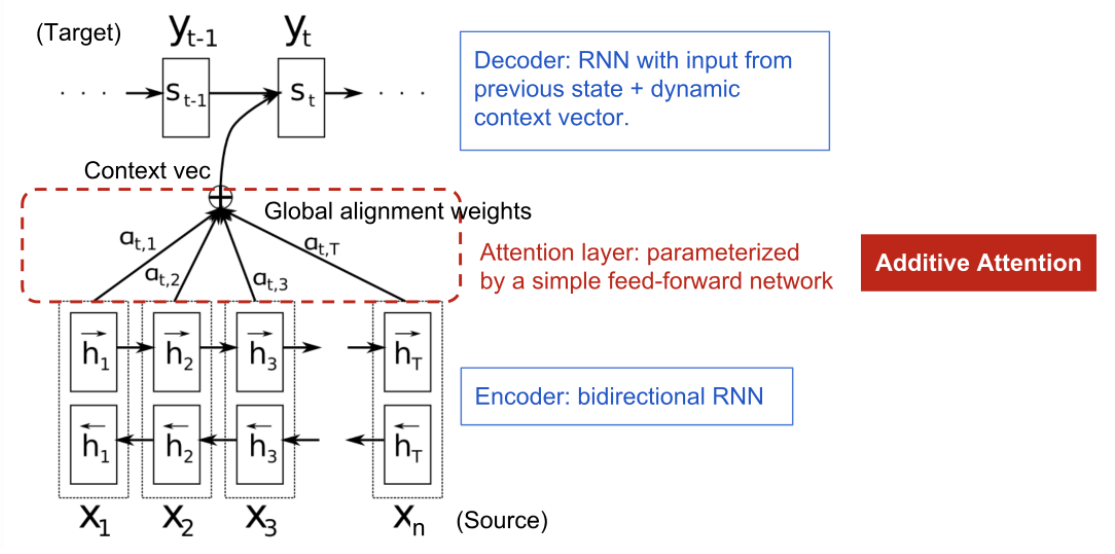
\includegraphics[width=0.8 \textwidth]{Chapters/1. Transformer/Figures/rnn/attention.png}
    \caption{Modelo seq2seq propuesto por Bahdanau et. al \cite{bahdanau2016neural} con \textit{Additive/Concat Attention}}
    \label{fig:att}
\end{figure}


Así, diversas investigaciones comenzaron surgir con distintos\textit{Mecanismo de Atención}. La tabla
\ref{Tab:att} resume estos métodos.

\begin{table}[]
\begin{center}
\begin{tabular}{@{}lll@{}}
\toprule
\textbf{Nombre} & \textbf{Función de Puntaje de Alineación} & \textbf{Cita} \\ \midrule
Content-Base Attention & $score(s^{(t)}, h^{(i)}) = cosine[s^{(t)}, h^{(i)}]$ & \cite[Graves 2014]{DBLP:journals/corr/GravesWD14} \\
Additive \textsuperscript{1} & $score(s^{(t)}, h^{(i)}) = v^\top_a \tanh(W_a[s^{(t)};h^{(i)}])$ &  \cite[Bahdanau 2015]{bahdanau2016neural}  \\
Location-Base & $a_{t,i} = softmax(W_a s^{(t)})$ & \cite[Luong 2015]{DBLP:journals/corr/LuongPM15} \\
General & $score(s^{(t)}, h^{(i)}) = s^{(t)\top} W_a h^{(i)}$ &  \cite[Luong 2015]{DBLP:journals/corr/LuongPM15} \\
Dot Product & $score(s^{(t)}, h^{(i)}) = s^{(t)\top} h^{(i)}$ &  \cite[Luong 2015]{DBLP:journals/corr/LuongPM15} \\
Scaled Dot-Product \textsuperscript{2} & $score(s^{(t)}, h^{(i)}) = \frac{s^{(t)\top} h^{(i)}}{\sqrt{d_k}}$ &  \cite[Vaswani 2017]{DBLP:journals/corr/VaswaniSPUJGKP17} \\ \bottomrule
\end{tabular}
\end{center}
\caption{Tipos de funciones para calcular el Puntaje de Alineación. (Tabla basada en \cite{weng2018attention}). \\
\textsuperscript{1} También llamado \textit{Concat} Luong, et al., 2015 y
\quotes{Additive attention”} en Vaswani, et al., 2017.\\
\textsuperscript{2} El factor de escala $\frac{1}{\sqrt{d_k}}$ ayuda a estabilizar cuando el
gradiente es muy pequeño. $d_k$ es el tamaño de la cabeza de atención.
\label{Tab:att}}
\end{table}
